\subsubsection{Caso d'uso UC8.1.3.4: Creazione domanda di collegamento}
\label{UC8.1.3.4}
\begin{figure}[h]
	\centering
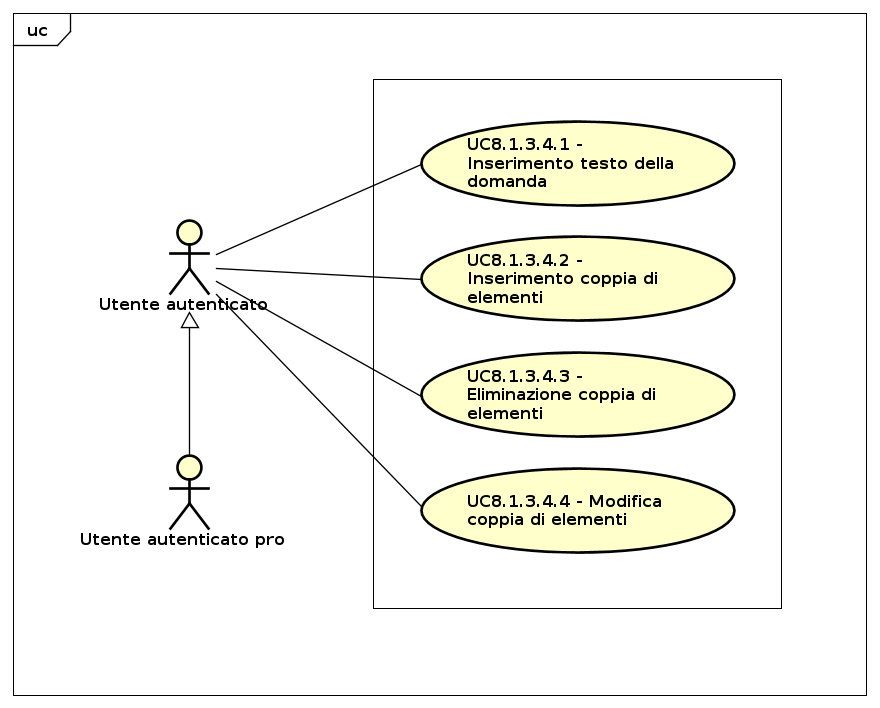
\includegraphics[scale=0.5,keepaspectratio]{UML/UC8_1_3_4.png}
	\caption{Caso d'uso UC8.1.3.4: Creazione domanda di collegamento}
\end{figure}
\FloatBarrier
\begin{itemize}
	\item \textbf{Attori}: \uau, \uaupro;
	\item \textbf{Descrizione}: l'attore utilizza la procedura guidata per la creazione di una domanda di tipo collegamento; 
	\item \textbf{Precondizione}: l'attore ha scelto l'opzione "Creazione domanda di collegamento" nelle scelte possibili nel caso d'uso UC8.1.3;
	\item \textbf{Postcondizione}: l'attore ha completato tutti i campi necessari per la creazione di una domanda di tipo collegamento. L'attore deve inserire almeno due coppie per rispettare la postcondizione;
	\item \textbf{Scenario principale}: 
		\begin{enumerate}
			\item L'attore inserisce una coppia di elementi (UC8.1.3.4.1);
			\item L'attore può eliminare una coppia di elementi appena inserita (UC8.1.3.4.2);
			\item L'attore può modificare una coppia di elementi (UC8.1.3.4.3);
			\item L'attore può inserire il testo della domanda (UC8.1.3.4.4).
		\end{enumerate}
	\item \textbf{Scenari alternativi}: se non ci sono almeno due coppie presenti nella lista delle coppie l'utente deve inserire una nuova coppia di elementi.
\end{itemize}

	\subsubsection{Caso d'uso UC8.1.3.4.1: Inserimento coppia di elementi}
	\label{UC8.1.3.4.1}
	\begin{figure}[h]
		\centering
		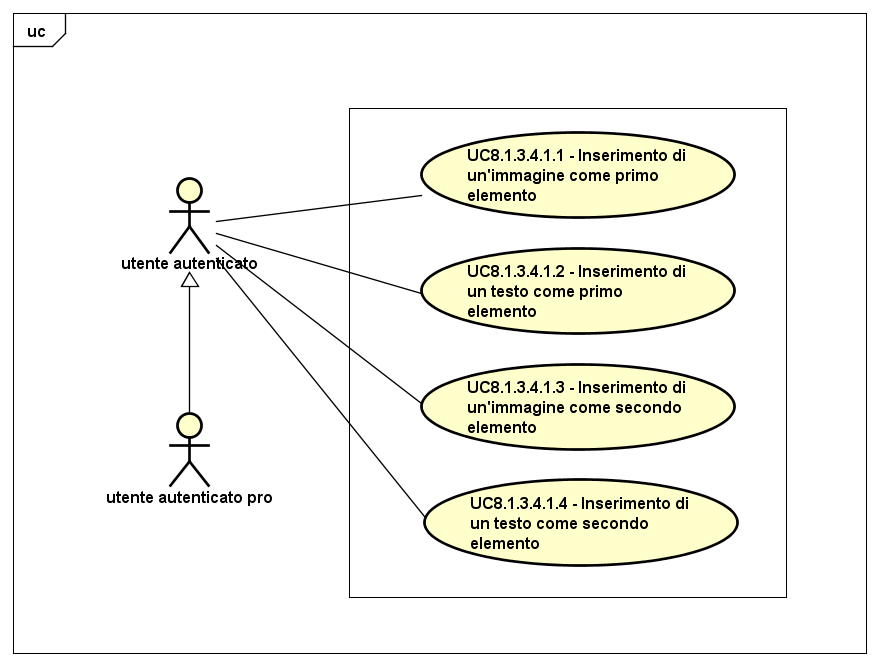
\includegraphics[scale=0.5,keepaspectratio]{UML/UC8_1_3_4_1.png}
		\caption{Caso d'uso UC8.1.3.4.1: Inserimento coppia di elementi}
	\end{figure}
	\FloatBarrier
	\begin{itemize}
		\item \textbf{Attori}: \uau, \uaupro;
		\item \textbf{Descrizione}: l'attore inserisce una coppia di elementi e questi possono essere sia immagini che testo o combinazioni di questi. Un coppia una volta creata sarà già soluzione di essa stessa: il primo elemento dovrà essere collegato con il secondo o viceversa; 
		\item \textbf{Precondizione}: l'attore ha scelto l'opzione "Inserimento coppia di elementi" nelle scelte possibili nel caso d'uso UC8.1.3.4;
		\item \textbf{Postcondizione}: l'attore ha inserito una coppia di elementi nella lista di coppie di elementi; 
		\item \textbf{Scenario principale}: 
		\begin{enumerate}
			\item L'attore inserisce come primo elemento un'immagine (UC8.1.3.4.1.1);
			\item L'attore inserisce come primo elemento un testo (UC8.1.3.4.1.2);
			\item L'attore inserisce come secondo elemento un'immagine (UC8.1.3.4.1.3);
			\item L'attore inserisce come secondo elemento un testo (UC8.1.3.4.1.4).	
		\end{enumerate}
	\end{itemize}
	
		\subsubsection{Caso d'uso UC8.1.3.4.1.1: Inserimento di un'immagine come primo elemento}
		\label{UC8.1.3.4.1.1}
		\begin{itemize}
			\item \textbf{Attori}: \uau, \uaupro;
			\item \textbf{Descrizione}: l'attore decide di inserire come primo elemento della coppia un'immagine;
			\item \textbf{Precondizione}: l'attore ha scelto l'opzione "Inserimento di un'immagine come primo elemento" nelle scelte possibili nel caso d'uso UC8.1.3.4.1 e non ha già scelto l'opzione presentata dall'use case UC8.1.3.4.1.2;
			\item \textbf{Postcondizione}: l'utente ha inserito come primo elemento un'immagine;
			\item \textbf{Scenario principale}: l'attore carica un'immagine come primo elemento della coppia;  
			\item \textbf{Scenari alternativi}: l'attore non può selezionare il seguente campo se è già stata utilizzata l'opzione proposta dall'use case UC8.1.3.4.1.2. Viene così rimandato all'use case UC8.1.3.4.1.
		\end{itemize}
		
		\subsubsection{Caso d'uso UC8.1.3.4.1.2: Inserimento di un testo come primo elemento}
		\label{UC8.1.3.4.1.2}
		\begin{itemize}
			\item \textbf{Attori}: \uau, \uaupro;
			\item \textbf{Descrizione}: l'attore decide di inserire come primo elemento della coppia un testo;
			\item \textbf{Precondizione}: l'attore ha scelto l'opzione "Inserimento di un testo come primo elemento" nelle scelte possibili nel caso d'uso UC8.1.3.4.1 e non ha già scelto l'opzione presentata dall'use case UC8.1.3.4.1.1;
			\item \textbf{Postcondizione}: l'utente ha inserito come primo elemento un testo;
			\item \textbf{Scenario principale}: l'attore inserisce del testo come primo elemento della coppia;  
			\item \textbf{Scenari alternativi}: l'attore non può selezionare il seguente campo se è già stata utilizzata l'opzione proposta dall'use case UC8.1.3.4.1.1. Viene così rimandato all'use case UC8.1.3.4.1.
		\end{itemize}
		
			\subsubsection{Caso d'uso UC8.1.3.4.1.3: Inserimento di un'immagine come secondo elemento}
		\label{UC8.1.3.4.1.3}
		\begin{itemize}
			\item \textbf{Attori}: \uau, \uaupro;
			\item \textbf{Descrizione}: l'attore decide di inserire come secondo elemento della coppia un'immagine;
			\item \textbf{Precondizione}: l'attore ha scelto l'opzione "Inserimento di un'immagine come secondo elemento" nelle scelte possibili nel caso d'uso UC8.1.3.4.1 e non ha già scelto l'opzione presentata dall'use case UC8.1.3.4.1.4;
			\item \textbf{Postcondizione}: l'utente ha inserito come secondo elemento un'immagine;
			\item \textbf{Scenario principale}: l'attore carica un'immagine come secondo elemento della coppia;  
			\item \textbf{Scenari alternativi}: l'attore non può selezionare il seguente campo se è già stata utilizzata l'opzione proposta dall'use case UC8.1.3.4.1.4. Viene così rimandato all'use case UC8.1.3.4.1.
		\end{itemize}
		
		\subsubsection{Caso d'uso UC8.1.3.4.1.4: Inserimento di un testo come secondo elemento}
		\label{UC8.1.3.4.1.4}
		\begin{itemize}
			\item \textbf{Attori}: \uau, \uaupro;
			\item \textbf{Descrizione}: l'attore decide di inserire come secondo elemento della coppia un testo;
			\item \textbf{Precondizione}: l'attore ha scelto l'opzione "Inserimento di un testo come secondo elemento" nelle scelte possibili nel caso d'uso UC8.1.3.4.1 e non ha già scelto l'opzione presentata dall'use case UC8.1.3.4.1.3;
			\item \textbf{Postcondizione}: l'utente ha inserito come secondo elemento un'immagine;
			\item \textbf{Scenario principale}: l'attore inserisce del testo come secondo elemento della coppia;  
			\item \textbf{Scenari alternativi}: l'attore non può selezionare il seguente campo se è già stata utilizzata l'opzione proposta dall'use case UC8.1.3.4.1.3. Viene così rimandato all'use case UC8.1.3.4.1.
		\end{itemize}
	
	\subsubsection{Caso d'uso UC8.1.3.4.2: Eliminazione coppia di elementi}
	\label{UC8.1.3.4.2}
	\begin{figure}[h]
		\centering
		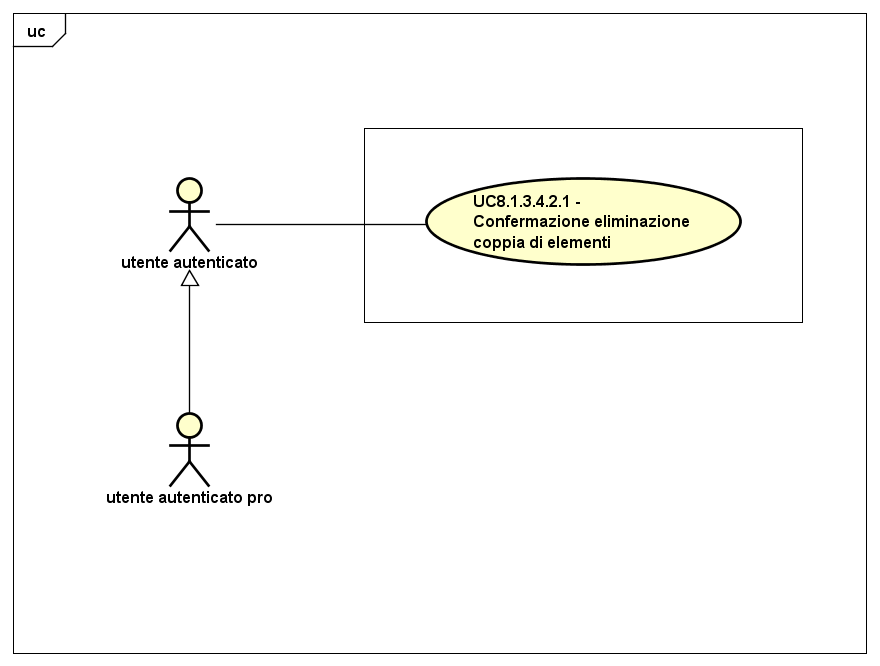
\includegraphics[scale=0.5,keepaspectratio]{UML/UC8_1_3_4_2.png}
		\caption{Caso d'uso UC8.1.3.4.2: Eliminazione coppia di elementi}
	\end{figure}
	\FloatBarrier
	\begin{itemize}
		\item \textbf{Attori}: \uau, \uaupro;
		\item \textbf{Descrizione}: l'utente decide di eliminare una coppia di elementi dalla lista di coppie di elementi;
		\item \textbf{Precondizione}: l'attore ha scelto l'opzione "Eliminazione coppia di elementi" nelle scelte possibili nel caso d'uso UC8.1.3.4;
		\item \textbf{Postcondizione}: l'attore ha eliminato, dalla lista delle coppie di elementi, una coppia;
		\item \textbf{Scenario principale}: l'attore deve confermare di voler eliminare una coppia di elementi (UC8.1.3.4.2.1).
	\end{itemize}

		\subsubsection{Caso d'uso UC8.1.3.4.2.1: Conferma eliminazione coppia di elementi}
		\label{UC8.1.3.4.2.1}
		\begin{itemize}
			\item \textbf{Attori}: \uau, \uaupro;
			\item \textbf{Descrizione}: l'attore deve confermare di voler eliminare la coppia di elementi;
			\item \textbf{Precondizione}: l'attore ha scelto l'opzione "Conferma eliminazione coppia di elementi" nelle scelte possibili nel caso d'uso UC8.1.3.4.2;
			\item \textbf{Postcondizione}: l'attore ha confermato di voler eliminare la coppia di elementi;
			\item \textbf{Scenario principale}: l'attore conferma di voler eliminare la coppia di elementi;
			\item \textbf{Scenari alternativi}: l'attore non conferma di voler eliminare la coppia di elementi.
		\end{itemize}

	\subsubsection{Caso d'uso UC8.1.3.4.3: Modifica coppia di elementi}
	\label{UC8.1.3.4.3}
	\begin{figure}[h]
		\centering
		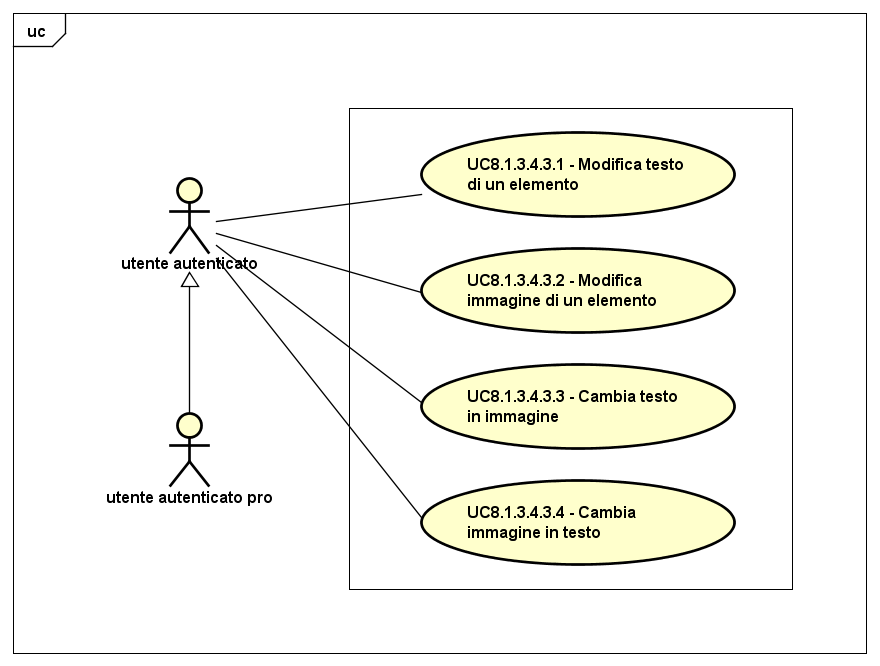
\includegraphics[scale=0.5,keepaspectratio]{UML/UC8_1_3_4_3.png}
		\caption{Caso d'uso UC8.1.3.4.3: Modifica coppia di elementi}
	\end{figure}
	\FloatBarrier
	\begin{itemize}
		\item \textbf{Attori}: \uau, \uaupro;
		\item \textbf{Descrizione}: l'attore modifica una coppia di elementi;
		\item \textbf{Precondizione}: l'attore ha scelto l'opzione "Modifica coppia di elementi" nelle scelte possibili nel caso d'uso UC8.1.3.4;
		\item \textbf{Postcondizione}: l'attore ha modificato una coppia di elementi nella lista di coppie di elementi; 
		\item \textbf{Scenario principale}: 
		\begin{enumerate}
			\item L'attore modifica un elemento cambiandone il testo (UC8.1.3.4.1.1);
			\item L'attore modifica un elemento cambiandone l'immagine (UC8.1.3.4.1.2);
			\item L'attore modifica un elemento facendolo passare da testo ad immagine (UC8.1.3.4.1.3);
			\item L'attore modifica un elemento facendolo passare da immagine a testo (UC8.1.3.4.1.4).	
		\end{enumerate}
	\end{itemize}
	
		\subsubsection{Caso d'uso UC8.1.3.4.3.1: Modifica testo di un elemento}
		\label{UC8.1.3.4.3.1}
		\begin{itemize}
			\item \textbf{Attori}: \uau, \uaupro;
			\item \textbf{Descrizione}: l'attore decide di modificare il testo di un elemento;
			\item \textbf{Precondizione}: l'attore ha scelto l'opzione "Modifica testo di un elemento" nelle scelte possibili nel caso d'uso UC8.1.3.4.3;
			\item \textbf{Postcondizione}: l'utente ha modificato il testo di un elemento;
			\item \textbf{Scenario principale}: l'attore modifica il testo di un elemento.  
		\end{itemize}
		
		\subsubsection{Caso d'uso UC8.1.3.4.3.2: Modifica immagine di un elemento}
		\label{UC8.1.3.4.3.2}
		\begin{itemize}
			\item \textbf{Attori}: \uau, \uaupro;
			\item \textbf{Descrizione}: l'attore decide di caricare un'altra immagine per un elemento;
			\item \textbf{Precondizione}: l'attore ha scelto l'opzione "Modifica immagine di un elemento" nelle scelte possibili nel caso d'uso UC8.1.3.4.3;
			\item \textbf{Postcondizione}: l'utente ha caricato un'altra immagine per un elemento;
			\item \textbf{Scenario principale}: l'attore carica un'altra immagine per un elemento.
		\end{itemize}
		
		\subsubsection{Caso d'uso UC8.1.3.4.3.3: Cambia testo in immagine}
		\label{UC8.1.3.4.3.3}
		\begin{itemize}
			\item \textbf{Attori}: \uau, \uaupro;
			\item \textbf{Descrizione}: l'attore decide di modificare un elemento facendolo diventare un'immagine al posto di un testo;
			\item \textbf{Precondizione}: l'attore ha scelto l'opzione "Cambia testo in immagine" nelle scelte possibili nel caso d'uso UC8.1.3.4.3;
			\item \textbf{Postcondizione}: l'utente ha fatto diventare un'immagine un elemento che prima era un testo;
			\item \textbf{Scenario principale}: l'attore inserisce un'immagine come modifica dell'elemento.  
		\end{itemize}
		
		\subsubsection{Caso d'uso UC8.1.3.4.3.4: Cambia immagine in testo}
		\label{UC8.1.3.4.3.4}
		\begin{itemize}
			\item \textbf{Attori}: \uau, \uaupro;
			\item \textbf{Descrizione}: l'attore decide di modificare un elemento facendolo diventare un testo al posto di un'immagine;
			\item \textbf{Precondizione}: l'attore ha scelto l'opzione "Cambia immagine in testo" nelle scelte possibili nel caso d'uso UC8.1.3.4.3;
			\item \textbf{Postcondizione}: l'utente ha fatto diventare un testo un elemento che prima era un'immagine;
			\item \textbf{Scenario principale}: l'attore inserisce del testo come modifica dell'elemento.  
		\end{itemize}
		
	\subsubsection{Caso d'uso UC8.1.3.4.4: Inserimento testo della domanda}
	\begin{itemize}
		\item
		\textbf{Attori}: \uau, \uaupro;
		\item		
		\textbf{Descrizione}: lo scopo di questa funzionalità è offrire all'attore la possibilità di inserire il testo della domanda;
		\item
		\textbf{Precondizione}: l'attore ha scelto l'opzione "Inserimento testo della domanda" nelle scelte possibili nel caso d'uso UC8.1.3.4.3;
		\item \textbf{Postcondizione}: l'attore ha inserito il testo della domanda;
		\item \textbf{Scenario principale}: l'attore inserisce il testo della domanda. 
	\end{itemize}
